%  Pt3.tex
% !TeX spellcheck = en_GB
% !TeX root = ProjectRiskManagement.tex
\section{The Evaluate Phase} \label{s:Evaluate}

For the evaluate phase of the PUMP approach, in the execution and delivery strategy shaping phase of a project’s lifecycle, explain concisely in your own words what you believe are the key features of a PUMP approach, comparing these features with the PMI PIMBOK approach or any other form of common practice you are familiar with. Your discussion should demonstrate your ability to understand a particular area of the course material in depth, based on selective reading, critical analysis and the case study exercise. Use examples to illustrate your discussion if you wish, and make use of the Transcon case study if you wish, but concentrate on concepts and principles. Build on your Parts 1 and 2 answers, avoiding repetition.

900 words.

\begin{figure}[!h]
  \centering
    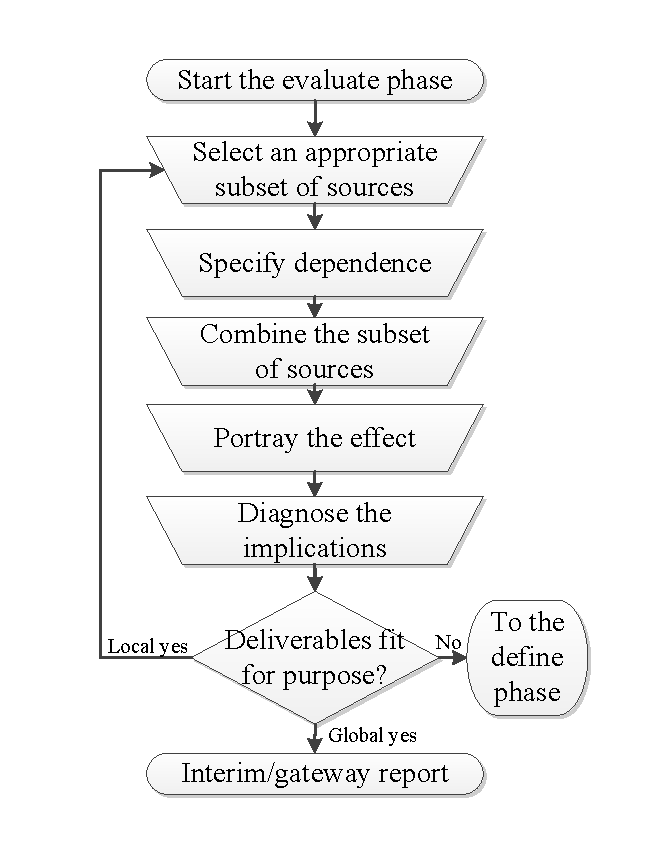
\includegraphics[width = 0.5\textwidth]{./Figures/Evaluate.pdf} 
\caption{Evaluate Phase Process - adapted from \cite{chapman}}
\label{Figure:Evaluate}
\end{figure}